\documentclass[Master.tex]{subfiles}
\begin{document}

%=======================================================%

\begin{frame}[fragile]
	\frametitle{Statistics with Julia}
	\large

\begin{verbatim}	
	plot(dataset("ggplot2", "diamonds"), 
	     x="Price", Geom.histogram)
\end{verbatim}
\begin{figure}
\centering
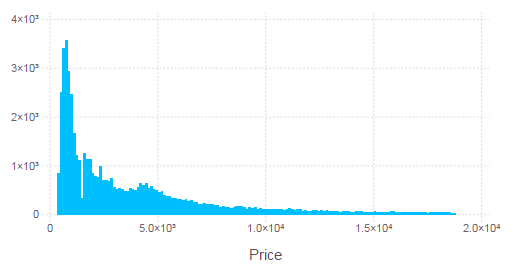
\includegraphics[width=0.95\linewidth]{images/histogram1}
\end{figure}

\end{frame}

%=======================================================%
\begin{frame}[fragile]
	\frametitle{Statistics with Julia}
	\large
\begin{verbatim}
plot(dataset("ggplot2", "diamonds"), 
	      x="Price", color="Cut", Geom.histogram)
\end{verbatim}
\begin{figure}
	\centering
	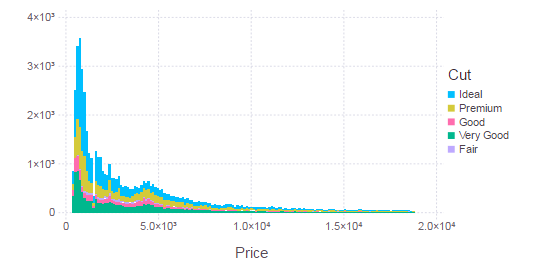
\includegraphics[width=0.95\linewidth]{images/histogram2}
\end{figure}
\end{frame}

%=======================================================%
\begin{frame}[fragile]
	\frametitle{Statistics with Julia}
	\large
\begin{verbatim}	
plot(dataset("ggplot2", "diamonds"), x="Price", 
	     color="Cut", Geom.histogram(bincount=30))
\end{verbatim}
\begin{figure}
	\centering
	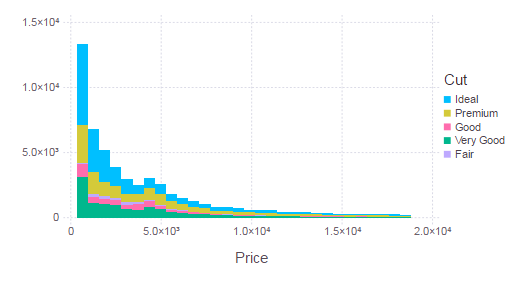
\includegraphics[width=0.95\linewidth]{images/histogram3}
\end{figure}
\end{frame}
%=======================================================%
\end{document}


